\section{Aufbau}

In diesem Versuch werden zwei Spektrallinien einer Cadmium-Lampe untersucht. Dabei dient die rote Linie zur Untersuchung des normalen Zeeman-Effekts und die blaue Linie dient zur Untersuchung des anomalen Effekts. Damit die Lampe ein Magnetfeld erfährt und dann die einzelnen Spektrallinien getrennt beobachtet werden können wird der Aufbau aus Abbildung \ref{fig:aufbau} genutzt.
\begin{figure}
  \centering
  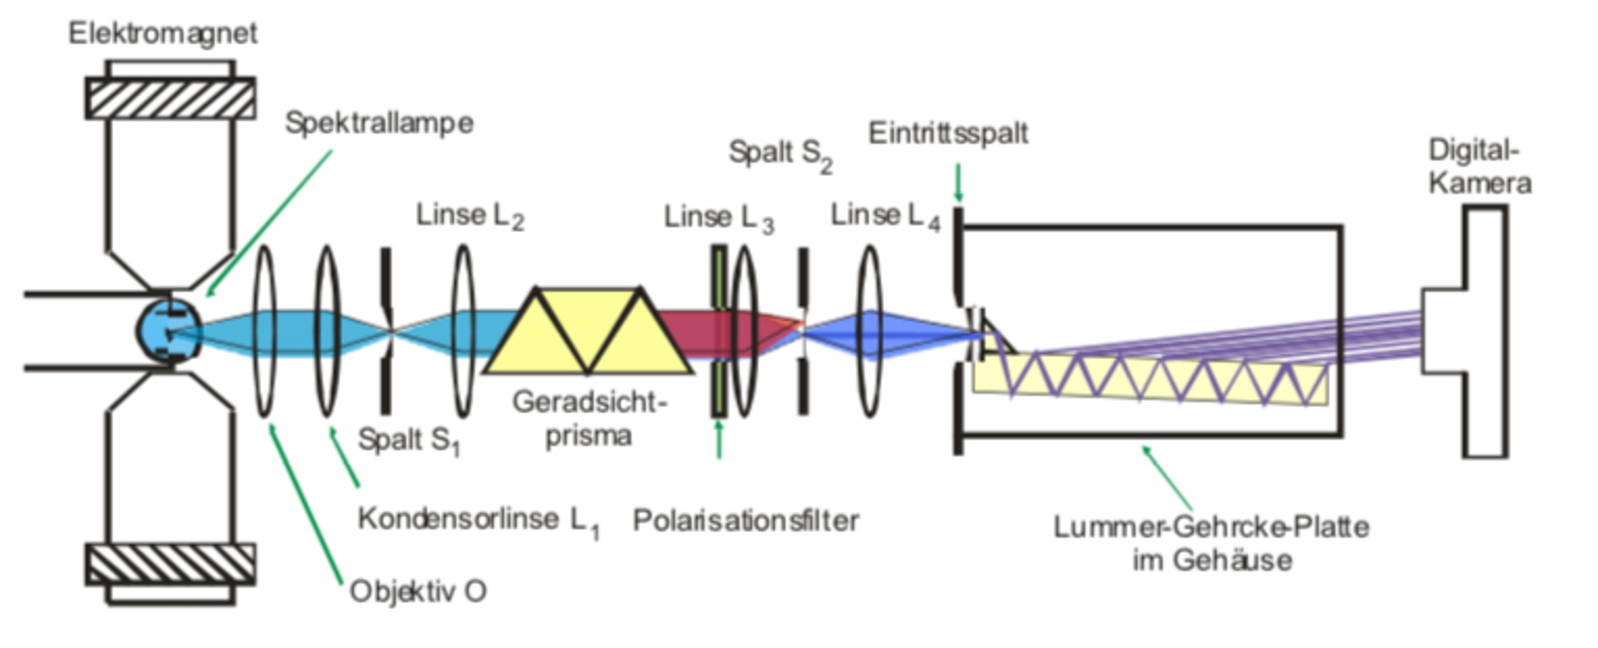
\includegraphics[height=6cm]{besuchInDerNacktmullAufzuchtstation/aufbau.pdf}
  \caption{Skizze des hier genutzten Versuchsaufbau \cite{anleitung}.}
  \label{fig:aufbau}
\end{figure}
Hier wird zunächst die Cadmium-Lampe zwischen einem Elektromagneten platziert, dessen Magnetfeld einstellbar ist. Das transversal zur Feldrichtung ausgesandte Licht wird dann durch Linsen und einen Spalt kollimiert auf ein Geradsichtprisma gelenkt. Dieses lenkt die verschiedenfarbigen Bestandteile des Lichts unterschiedlich stark ab, sodass mithilfe des dahinter platzierten Spalts eine Spektrallinie ausgesucht werden kann. Die Linie wird dann fokussiert auf eine Lummer-Gehrcke-Platte geleitet. Darin wird  es wiederholt zwischen beiden Seiten der Platte reflektiert. Bei jeder Reflektion kann Licht austreten und mit den anderen austretenden Strahlen interferieren. Für konstruktive Interferenz gilt
die Beziehung:
\begin{align}
  2 d \cos(\theta) = n \lambda.
\end{align}
Wobei $d$ die Dicke der Platte, $\theta$ der Beobachtungswinkel, $n$ die Ordnung der Interferenz und $\lambda$ die Wellenlänge ist. Mit der Digitalkamera können dann Interferenzstreifen aufgenommen werden, dessen Gangunterschied genau die Wellenlänge ist. Das Magnetfeld verschiebt die Wellenlänge um $\delta \lambda$ wodurch sich die Lage der Interferenzstreifen um $\delta s$ verändert.
Zusätzlich wird ein Polarisationsfilter an einer beliebigen Stelle in dem Aufbau platziert um, je nachdem ob die $\pi$-Linie oder $\sigma$-Linie beobachtet wird, nur diese Polarisation durchzulassen.
Das Dispersionsgebiet
der LG-Platte ist
\begin{align}
  \Delta \lambda_\text{D} = \frac{\lambda^2}{2 d} \sqrt{\frac{1}{n^2-1}}.
\end{align}
Es gibt an, wie groß die maximale Wellenlängendifferenz sein darf, bevor sich zwei Wellenlängen überlagern. Außerdem kann man das Auflösungsvermögen der Platte mit
\begin{align}
  A = \frac{\lambda}{\Delta \lambda} = \frac{L}{\lambda} (n^2 - 1)
\end{align}
beschreiben.

Die Wellenlängen der roten und blauen Linie betragen:
\begin{align*}
  \lambda_\text{rot} &= \SI{643.8}{\nano\meter} \quad \lambda_\text{blau} = \SI{480.0}{\nano\meter}.\\
\intertext{Und die Werte der LG-Platte betragen:}
  d &= \SI{4}{\milli\meter} \quad L = \SI{120}{\milli\meter} \quad n(\SI{644}{\nano\meter}) = \num{1.4567} \quad n(\SI{480}{\nano\meter}) = \num{1.4635}.
\end{align*}

\section{Durchführung}
\label{sec:Durchführung}

Zu Beginn wird mithilfe einer Hall-Sonde eine Kalibrationsmessung des Elektromagneten durchgeführt. Hierzu wird das Magnetfeld in Abhängigkeit von der eingestellten Stromstärke gemessen.

Als nächstes muss der optische Weg justiert werden.
Dazu werden als Erstes die ersten drei Linsen und der Spalt so postiert, dass ein paralleles Lichtbündel auf das Prisma fällt. Außerdem wird darauf geachtet, dass die Linien, die nach dem Prisma und der Linse $L_3$ auf den Spalt treffen möglichst hell, scharf und parallel zur Spaltöffnung sind. Die durch den Spalt bestimmte Spektrallinie sollte dann genau auf die Öffnung der LG-Platte treffen. Das kann mit $L_4$ eingestellt werden. Nach diesen Schritten und der geeigneten Platzierung und Fokussierung der Digitalkamera kann dort ein Interferenzbild aufgenommen werden.

Begonnen wird nun mit der roten Linie. Hier wird erst ein Bild ohne Magnetfeld aufgenommen, als Referenz für die Ablenkung. Dann wird das zuvor berechnete Magnetfeld eingestellt, dass ein möglichst überlagerungsfreies Bild der $\sigma$-Aufspaltung ergibt. Hiervon wird ebenfalls ein Bild mit der Kamera aufgenommen.
Anschließend wird bei der blauen Linie ähnlich verfahren. Der Unterschied ist hier, dass die $\pi$-Linie ebenfalls aufspaltet und deshalb zwei verschieden starke Magnetfelder eingestellt werden müssen. Welche Linie gerade untersucht wird, kann über den Polarisationsfilter eingestellt werden.
